\begin{notecard}{Ángulos entre una secante y dos rectas paralelas}
    \begin{tcbitemize}[%
            raster columns=3,
            raster equal height,
            raster equal skip=0pt,
            raster column skip=0pt,
            size=small,
            sharpish corners,
            colback=MainColor!2!white,
            colframe=MainColor!50!white,
            colbacktitle=MainColor!20!white,
            center title,
            coltitle=black,
            fonttitle=\small]
        \captionsetup[figure]{labelformat=empty,font={small}}% redefines the caption setup of the figures
        \tcbitem[adjusted title={Ángulos Colaterales}]
        \begin{figure}[H]
            \centering
            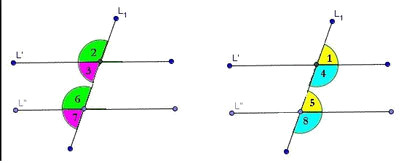
\includegraphics[width=\linewidth]{../images/angulos_colaterales}
            \caption{Son los ángulos que están ubicados al mismo lado de la secante.}
            \label{fig:angulos_colaterales}
        \end{figure}
        \tcbitem[adjusted title={Ángulos Internos}]
        \begin{figure}[H]
            \centering
            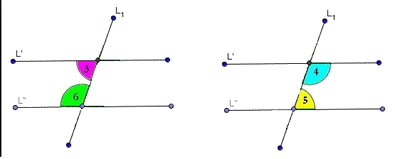
\includegraphics[width=\linewidth]{../images/angulos_internos}
            \caption{Son los ángulos que están ubicados entre las rectas paralelas.}
            \label{fig:angulos_internos}
        \end{figure}
        \tcbitem[adjusted title={Ángulos Externos}]
        \begin{figure}[H]
            \centering
            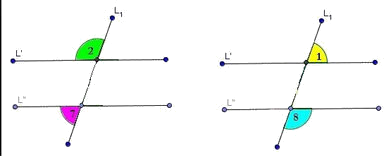
\includegraphics[width=\linewidth]{../images/angulos_externos}
            \caption{Son los ángulos que están ubicados por fuera de las rectas paralelas.}
            \label{fig:angulos_externos}
        \end{figure}
        \tcbitem[adjusted title={Ángulos Alternos Internos}]
        \begin{figure}[H]
            \centering
            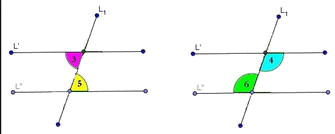
\includegraphics[width=\linewidth]{../images/angulos_alternos_internos}
            \caption{Son dos ángulos internos que no son colaterales ni adyacentes.}
            \label{fig:angulos_alternos_internos}
        \end{figure}
        \tcbitem[adjusted title={Ángulo Alternos Externos}]
        \begin{figure}[H]
            \centering
            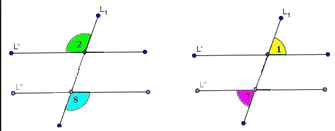
\includegraphics[width=\linewidth]{../images/angulos_alternos_externos}
            \caption{Son dos ángulos externos que no son colaterales ni adyacentes.}
            \label{fig:angulos_alternos_externos}
        \end{figure}
        \tcbitem[adjusted title={Ángulos Correspondientes}]
        \begin{figure}[H]
            \centering
            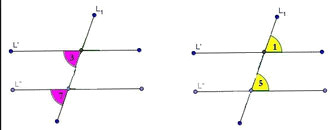
\includegraphics[width=\linewidth]{../images/angulos_correspondientes}
            \caption{Son dos ángulos uno interno y el otro externo que son colaterales pero no adyacentes.}
            \label{fig:angulos_correspondientes}
        \end{figure}
    \end{tcbitemize}
\end{notecard}